\documentclass[border=10pt]{standalone}
\usepackage{tikz,amsmath,amssymb}
\usetikzlibrary{arrows.meta}
\usepackage{tikzcats}   % 原生保留 tikzcats

% ========== 配色方案 ==========
\definecolor{inFill}{RGB}{183,224,177}       % 浅绿 (早期浅层特征)
\definecolor{inLine}{RGB}{32,102,32}
\definecolor{orFill}{RGB}{250,224,180}      % 橙黄 (中层语义特征)
\definecolor{orLine}{RGB}{190,110,20}
\definecolor{yeFill}{RGB}{252,240,180}      % 鹅黄 (深层高度抽象特征)
\definecolor{yeLine}{RGB}{180,150,20}
\definecolor{hidFill}{RGB}{199,203,243}     % 紫蓝 (FC 全连接特征向量)
\definecolor{hidLine}{RGB}{52,58,143}
\definecolor{outFill}{RGB}{243,199,199}     % 红色系 (目标类别高亮)
\definecolor{outLine}{RGB}{143,52,52}
\definecolor{gyFill}{RGB}{235,235,238}      % 浅灰 (非目标类别)
\definecolor{gyLine}{RGB}{140,140,145}

\begin{document}
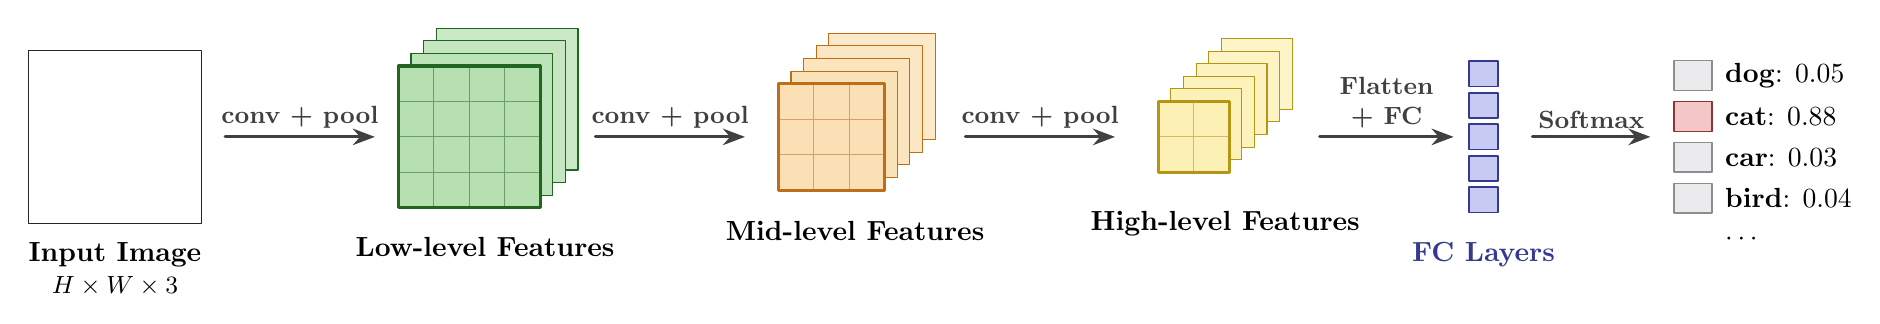
\begin{tikzpicture}[
    font=\normalsize, line join=round, line cap=round,
    every node/.style={inner sep=0pt, outer sep=0pt, align=center},
    arr/.style={->, >=Stealth, line width=1.1pt, darkgray}
  ]

  % ========== 宏：优化后的 3D 堆叠特征图 ==========
  % 背后层：采用纯色填充与细腻描边表现纵深；最前面一层：高清网格与加粗轮廓
  % #1: x中心, #2: y中心, #3: 堆叠层数, #4: 网格数, #5: 单格尺寸, #6: 颜色前缀
  \newcommand{\fstack}[6]{%
    \pgfmathsetmacro{\sz}{#4*#5}
    \pgfmathsetmacro{\half}{\sz/2}
    % 背后深度切片 (平滑渐变无杂线)
    \foreach \k in {#3,...,1}{%
      \pgfmathtruncatemacro{\op}{round(100 - (28 * \k / #3))}
      \fill[#6Fill!\op, draw=#6Line, line width=.4pt]
        ({#1 - \half + 0.16*\k}, {#2 - \half + 0.16*\k}) rectangle ++({\sz}, {\sz});
    }
    % 正面清晰网格切片
    \fill[#6Fill] ({#1 - \half}, {#2 - \half}) rectangle ++({\sz}, {\sz});
    \draw[step=#5, #6Line!65, line width=.35pt, shift={({#1 - \half}, {#2 - \half})}] (0,0) grid ({\sz}, {\sz});
    \draw[#6Line, line width=1.1pt] ({#1 - \half}, {#2 - \half}) rectangle ++({\sz}, {\sz});
  }

  % 输入猫咪图片 (2.2 x 2.2 cm, 中心严格置于 (1.1, 2.2))
  \newcommand{\catimg}[2]{%
    \draw[black!85, line width=.5pt, fill=white] ({#1-1.1},{#2-1.1}) rectangle ++(2.2,2.2);
    \node at (#1, #2) {\scalebox{0.185}{\tikz{\cat}}};
  }

  % 主架构流水线：水平中心严格统一对齐在 Y = 2.2
  % 1. 输入原图
  \catimg{1.1}{2.2}
  \node[font={\normalsize\bfseries}] at (1.1, 0.7) {Input Image};
  \node[font=\small, text=black] at (1.1, 0.3) {\(H\times W\times 3\)};

  % 2. 卷积 + 池化阶段 1 (低层特征)
  \draw[arr] (2.5, 2.2) -- (4.4, 2.2) node[midway, above=3pt, font={\small\bfseries}] {conv + pool};
  \fstack{5.6}{2.2}{3}{4}{0.45}{in}
  \node[font={\normalsize\bfseries}] at (5.8, 0.8) {Low-level Features};

  % 3. 卷积 + 池化阶段 2 (中层特征)
  \draw[arr] (7.2, 2.2) -- (9.1, 2.2) node[midway, above=3pt, font={\small\bfseries}] {conv + pool};
  \fstack{10.2}{2.2}{4}{3}{0.45}{or}
  \node[font={\normalsize\bfseries}] at (10.5, 1.0) {Mid-level Features};

  % 4. 卷积 + 池化阶段 3 (高层特征)
  \draw[arr] (11.9, 2.2) -- (13.8, 2.2) node[midway, above=3pt, font={\small\bfseries}] {conv + pool};
  \fstack{14.8}{2.2}{5}{2}{0.45}{ye}
  \node[font={\normalsize\bfseries}] at (15.2, 1.1) {High-level Features};

  % 5. 展平与全连接 (Flatten + FC)
  \draw[arr] (16.4, 2.2) -- (18.1, 2.2) node[midway, above=3pt, font={\small\bfseries}] {Flatten\\+ FC};

  % 垂直排列的 1D 全连接特征向量 (居中在 Y = 2.2)
  \foreach \i in {0,...,4}{%
    \fill[hidFill, draw=hidLine, line width=.6pt] (18.3, {1.24 + 0.40*\i}) rectangle ++(0.36, 0.32);
  }
  \node[font={\normalsize\bfseries}, text=hidLine] at (18.48, 0.7) {FC Layers};

  % 6. 分类预测 (Softmax 概率分布)
  \draw[arr] (19.1, 2.2) -- (20.6, 2.2) node[midway, above=3pt, font={\small\bfseries}] {Softmax};

  % 类别输出概率条 (居中在 Y = 2.2)
  \foreach \val/\col/\lbl [count=\i from 0] in {0.05/gy/dog, 0.88/out/cat, 0.03/gy/car, 0.04/gy/bird}{%
    \fill[\col Fill, draw=\col Line, line width=.6pt] (20.9, {2.79 - 0.52*\i}) rectangle ++(0.48, 0.38);
    \node[font=\normalsize, anchor=west] at (21.55, {2.98 - 0.52*\i}) {\textbf{\lbl}: \val};
  }

  % 下方添加 \cdots 表示多类别省略
  \node[font=\normalsize, anchor=west] at (21.55, {2.98 - 0.52*4}) {\(\cdots\)};

\end{tikzpicture}
\end{document}